\documentclass{article}

\usepackage{amsmath, microtype, physics, tikz, gensymb, cancel}
\usepackage{enumitem, float}
\usepackage[letterpaper, bottom=1in, top=1in, left=1in, right=1in]{geometry}

\usetikzlibrary{calc}

\newcommand{\x}{\mathrm{x}}
\newcommand{\y}{\mathrm{y}}
\newcommand{\z}{\mathrm{z}}
\newcommand{\ddt}[1]{\frac{\mathrm{d}}{\mathrm{d}t}[#1]}

\title{Homework Problem \#48}
\author{Laith}
\date{2/7/2023}

\begin{document}
\maketitle

\section*{Problem}
In Fig. 4-41, a ball is thrown up onto
a roof, landing 4.00 s later at height $h=20.0$ m 
above the release level. The ball's path just before 
landing is angled at $\theta=60.0\degree$ with the 
roof. 
\begin{enumerate}[label=(\alph*)]
    \item Find the horizontal distance $d$ it travels. 
    (See the hint to Problem 39.)
    \item What is the magnitude relative to the horizontal 
    of the ball's initial velocity?
    \item What is the angle relative to the horizontal of the 
    ball's initial velocity?
\end{enumerate}

\begin{figure}[H]
    \centering
    \caption{Figure 4-11}
    \begin{tikzpicture}
        \draw[dashed] (-1, 0) -- (10, 0);

        \draw[dashed, -stealth, very thick, red] (0, 0) .. controls (2, 5) and (4, 6) .. (6.5, 3);

        \draw[solid] (5, 3) -- (8, 3);
        \draw[solid] (5, 0) -- (5, 3);
        \draw[solid] (8, 0) -- (8, 3);

        \draw[stealth-] (6.5, 0) -- (6.5, 1);
        \node at (6.5, 1.5) {$h$};
        \draw[-stealth] (6.5, 2) -- (6.5, 3);

        \draw (0, -2) -- (0, -1);
        \draw (6.5, -2) -- (6.5, -1);

        \draw[stealth-]  (0, -1.5) -- (3, -1.5);
        \node at (3.25, -1.5) {$d$};
        \draw[-stealth]  (3.5, -1.5) -- (6.5, -1.5);

        \draw (6.5, 3) -- (5.9, 4);

        \draw (6.2, 3.5) arc (-270:-180:0.5) node[above left, yshift=5, xshift=2] {$\theta$};

        \draw (0.32, 0.8) arc (-270:-369:0.7) node[above right, yshift=10, xshift=-5] {$\theta_2$};
        \draw (0, 0) -- (0.8, 2); 

    \end{tikzpicture} 
\end{figure}

\newpage
\section*{Solution}

\subsection*{Part (a)}
In order to find distance $d$, we can define a function as the
horizontal position of the ball relative to where the ball landed.
In other words, this function will tell us the position of the ball
starting from the top of the building back to the ground. 

In order to define this fucntion, let's draw a right triangle using $\theta$:
\begin{figure}[H]
    \centering
    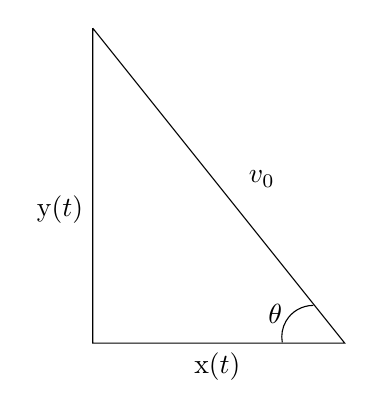
\begin{tikzpicture}[scale=0.8]
        \draw (0, 5) -- (0, 0) -- (4, 0) -- (0, 5);

        \draw (3.5, 0.6) arc (-270:-170:0.5) node[midway, xshift=-5, yshift=1] {$\theta$};

        \node[below left] at (0, 2.5) {$\y(t)$};
        \node[below left] at (2.5, 0) {$\x(t)$};

        \node[above right, xshift=-4, yshift=-4] at (2.5, 2.5) {$v_0$};
    \end{tikzpicture} 
\end{figure}
We can use $\cos(\theta)$ to solve for $\x(t)$, 
in which we multiply by time $t$ to cancel out initial velocity $v_0$:
\begin{align}
    \cos(\theta)  = \frac{\x(t)}{v_0} \Rightarrow \boxed{\x(t) = v_0\cos(\theta)t}
\end{align}

We can use $\sin(\theta)$ to solve for $\y(t)$,
where we also multiply by $t$ to cancel out velocity, 
but also subtract $\frac{1}{2}gt^2$ in order to account 
for gravity:
\begin{align}
    \sin(\theta) = \frac{\y(t)}{v_0} \Rightarrow \boxed{\y(t) = v_0\cos(\theta)t - \frac{1}{2}gt^2}
\end{align}

The reason we also need a function for the vertical position $\y(t)$
is that we have an undefined variable $v_0$, which means we cannot yet 
solve for $d$.

Since we know that the ball lands at a height $h=20$, we can say that
our function $\y(t)$ at time $t=4$ would equal $-20$:
\[
\begin{array}{lcl}
\begin{aligned}[t]
    \y(4) &= -20 \\
    \y(4) &= v_0\sin(60)(4)-\frac{1}{2}(10)(4)^2 \\
      -20 &= v_0\sin(60)(4)-\frac{1}{2}(10)(4)^2 \\
      -20 &= v_0\cancelto{2\sqrt3}{\frac{\sqrt3}{2}(4)}-\cancelto{5}{\frac{1}{2}(10)}(16) \\
      -20 &= v_02\sqrt3-80 \\
\end{aligned}
\hspace{1em}\vline\hspace{1em}
\begin{aligned}[t]
    \Rightarrow v_0 &= \frac{\cancelto{30}{60}}{\cancel{2}\sqrt3} \\
    \Rightarrow v_0 &= \frac{30\cdot \sqrt3}{\sqrt3 \cdot \sqrt3} \\
    \Rightarrow v_0 &= \frac{\cancelto{10}{30}\sqrt3}{\cancel{3}} = 10\sqrt3
\end{aligned}
\end{array}
\]
Now that we have $v_0=10\sqrt3$, we can now solve for $d$:
\[
    \begin{aligned}[t]
            d &= \x(4) \\
        \x(4) &= \cancelto{10\sqrt3}{v_0}\cos(60)(4) \\
\Rightarrow d &= (10\sqrt3)\cos(60)(4) \\
    \end{aligned}
    \hspace{1em}\vline\hspace{1em}
    \begin{aligned}[t]
            d &= (10\sqrt3)\cancelto{2}{\frac{1}{2}{4}} \\
            d &= (10\sqrt3)2  \\
            d &= 20\sqrt3 
    \end{aligned}
\]
Thus, the horizontal distance $d$ traveled by the ball is 
$20\sqrt3$ meters.

\newpage
\subsection*{Part (b)}
In order to find the magnitude of the initial velocity, we need 
to consider two things:
\begin{enumerate}
    \item What is velocity in this scenario?
    \item What functions can we use to model velocity?
\end{enumerate}
Velocity will be a 2D vector (if you made it 3D, the $z$-component
would just be 0 and have no effect on the magnitude):
\[ \abs{\va{V}} = (V_x,\, V_y) \]
Considering that, in terms of calculus, velocity is the derivative
of position, we can derive the two functions $\x(t)$ and $\y(t)$
with respect to $t$ to get the components of velocity respectively:
\[
    \begin{array}{lcl}    
        \begin{aligned}[t]
            V_x(t) &= \ddt{\x(t)} \\
            V_x(t) &= \ddt{10\sqrt3\frac{1}{2}t} \\
            V_x(t) &= \ddt{5\sqrt3\,t} \\
            V_x(t) &= 5\sqrt3 \\
            \rightarrow V_x &= 5\sqrt3
        \end{aligned}
        \hspace{1em}\vline\hspace{1em}
        \begin{aligned}[t]
           V_y(t) &= \ddt{\y(t)} \\
           V_y(t) &= \ddt{10\sqrt3\frac{\sqrt3}{2}t-\frac{1}{2}gt^2} \\
           V_y(t) &= \ddt{5\cdot3t-\frac{1}{2}(10)t^2} \\
           V_y(t) &= \ddt{15t-5t^2} \\
           V_y(t) &= 15-10t
        \end{aligned}
    \end{array}
\] 
Now we can solve for $V_y$ at time $t=4$. Keep in mind that the functions 
we derived from start at where the ball landed, which occured at 4 seconds 
after the ball was launched. The value of these functions at $t=4$ will 
still be the same as the functions starting from the ground at $t=0$:
\[
    \begin{array}{lcl}    
        \begin{aligned}[t]
           V_y(4) &= 15-10(4) \\
           V_y(4) &= 15-40 = -25 \\
           V_y(4) &= -25
        \end{aligned}
    \end{array}
\] 
Now we can calculate the magnitude of the initial velocity, in which 
we know that the magnitude of a vector is the square root of the 
sum of the squared components:
\[ \abs{\va{V}} = \sqrt{{V_x}^2+{V_y}^2} \]
So plugging in our values:
\begin{align*}
    \abs{\va{V}} &= \sqrt{{5\sqrt3}^2+{-25}^2} \\
                 &= \sqrt{25\cdot3+625} \\
                 &= \sqrt{75+625} = \sqrt{700} \\
                 &= \sqrt{100}\sqrt{7}
\end{align*}
Thus the magnitude of our initial velocity is:
\[ \boxed{\abs{\va{V}} = 10\sqrt{7}\,\mathrm{m/s}} \]

\newpage 
\subsection*{Part (c)}
We will designate $\theta_2$ to be the angle of the initial
velocity vector, and using that angle, we will draw a right 
triangle:
\begin{figure}[H]
    \centering
    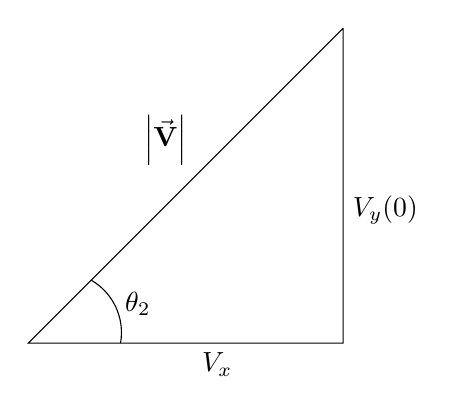
\begin{tikzpicture}[scale=0.8]
        \draw (5, 5) -- (5, 0) -- (0, 0) -- (5, 5);

        \draw (1, 1) arc (-300:-370:0.96) node[midway, xshift=8, yshift=1] {$\theta_2$};

        \node[below right] at (5, 2.5) {$V_y(0)$};
        \node[below] at (3, 0) {$V_x$};

        \node[above left, xshift=4, yshift=4] at (2.5, 2.5) {$\abs{\va{V}}$};
    \end{tikzpicture} 
\end{figure}
We can solve for $\theta_2$ using any of the trig functions, but
they key is to pass the value we get for the trig function into 
its respective inverse function:
{\footnotesize
\[
    \begin{array}{lcl}
        \begin{aligned}[t]
            \abs{\arctan(\tan(\theta_2))} &= \abs{\arctan(\frac{V_y(0)}{V_x})} \\
            \\
            &= \abs{\arctan(\frac{-25}{5\sqrt3})} \\
            \\
            &= \abs{\arctan(\frac{-5}{\sqrt3})} \\
            \\
            &\approx 70.89\degree\:*_\mathrm{Using\:a\:calculator.}
        \end{aligned} 
        \hspace{1em}\vline\hspace{1em}
        \begin{aligned}[t]
            \abs{\arcsin(\sin(\theta_2))} &= \abs{\arcsin(\frac{V_y(0)}{\abs{\va{V}}})} \\
            \\
            &= \abs{\arcsin(\frac{-25}{10\sqrt7})} \\
            \\
            &= \abs{\arcsin(\frac{-5}{2\sqrt7})} \\
            \\
            &\approx 70.89\degree\:*_\mathrm{Using\:a\:calculator.}
        \end{aligned} 
        \hspace{1em}\vline\hspace{1em}
        \begin{aligned}[t]
            \abs{\arccos(\cos(\theta_2))} &= \abs{\arccos(\frac{V_x}{v_0})} \\
            \\
            &= \abs{\arccos(\frac{5\sqrt3}{10\sqrt7})} \\
            \\
            &= \abs{\arccos(\frac{\sqrt3}{2\sqrt7})} \\
            \\
            &\approx 70.89\degree\:*_\mathrm{Using\:a\:calculator.}
        \end{aligned} 
    \end{array}
\]}
Thus, the magnitude of the angle of our initial velocity is $70.89\degree$.


\end{document}